\documentclass[11pt,a4paper]{ltjsarticle}
\usepackage{graphicx}
\usepackage{amsmath}
\usepackage{booktabs}
\usepackage[margin=22mm]{geometry}
\usepackage{xcolor}
\graphicspath{{./figures/}{./figures/pce_uq/}}

\title{\bfseries 確率有限要素法によるH3フェアリングの\\製造ばらつき信頼性評価（簡易要約）}
\author{西岡 佳祐 \quad（LUH 確率有限要素法 SoSe\,2026）}
\date{}

\begin{document}
\maketitle
\vspace{-1.5em}

\begin{center}
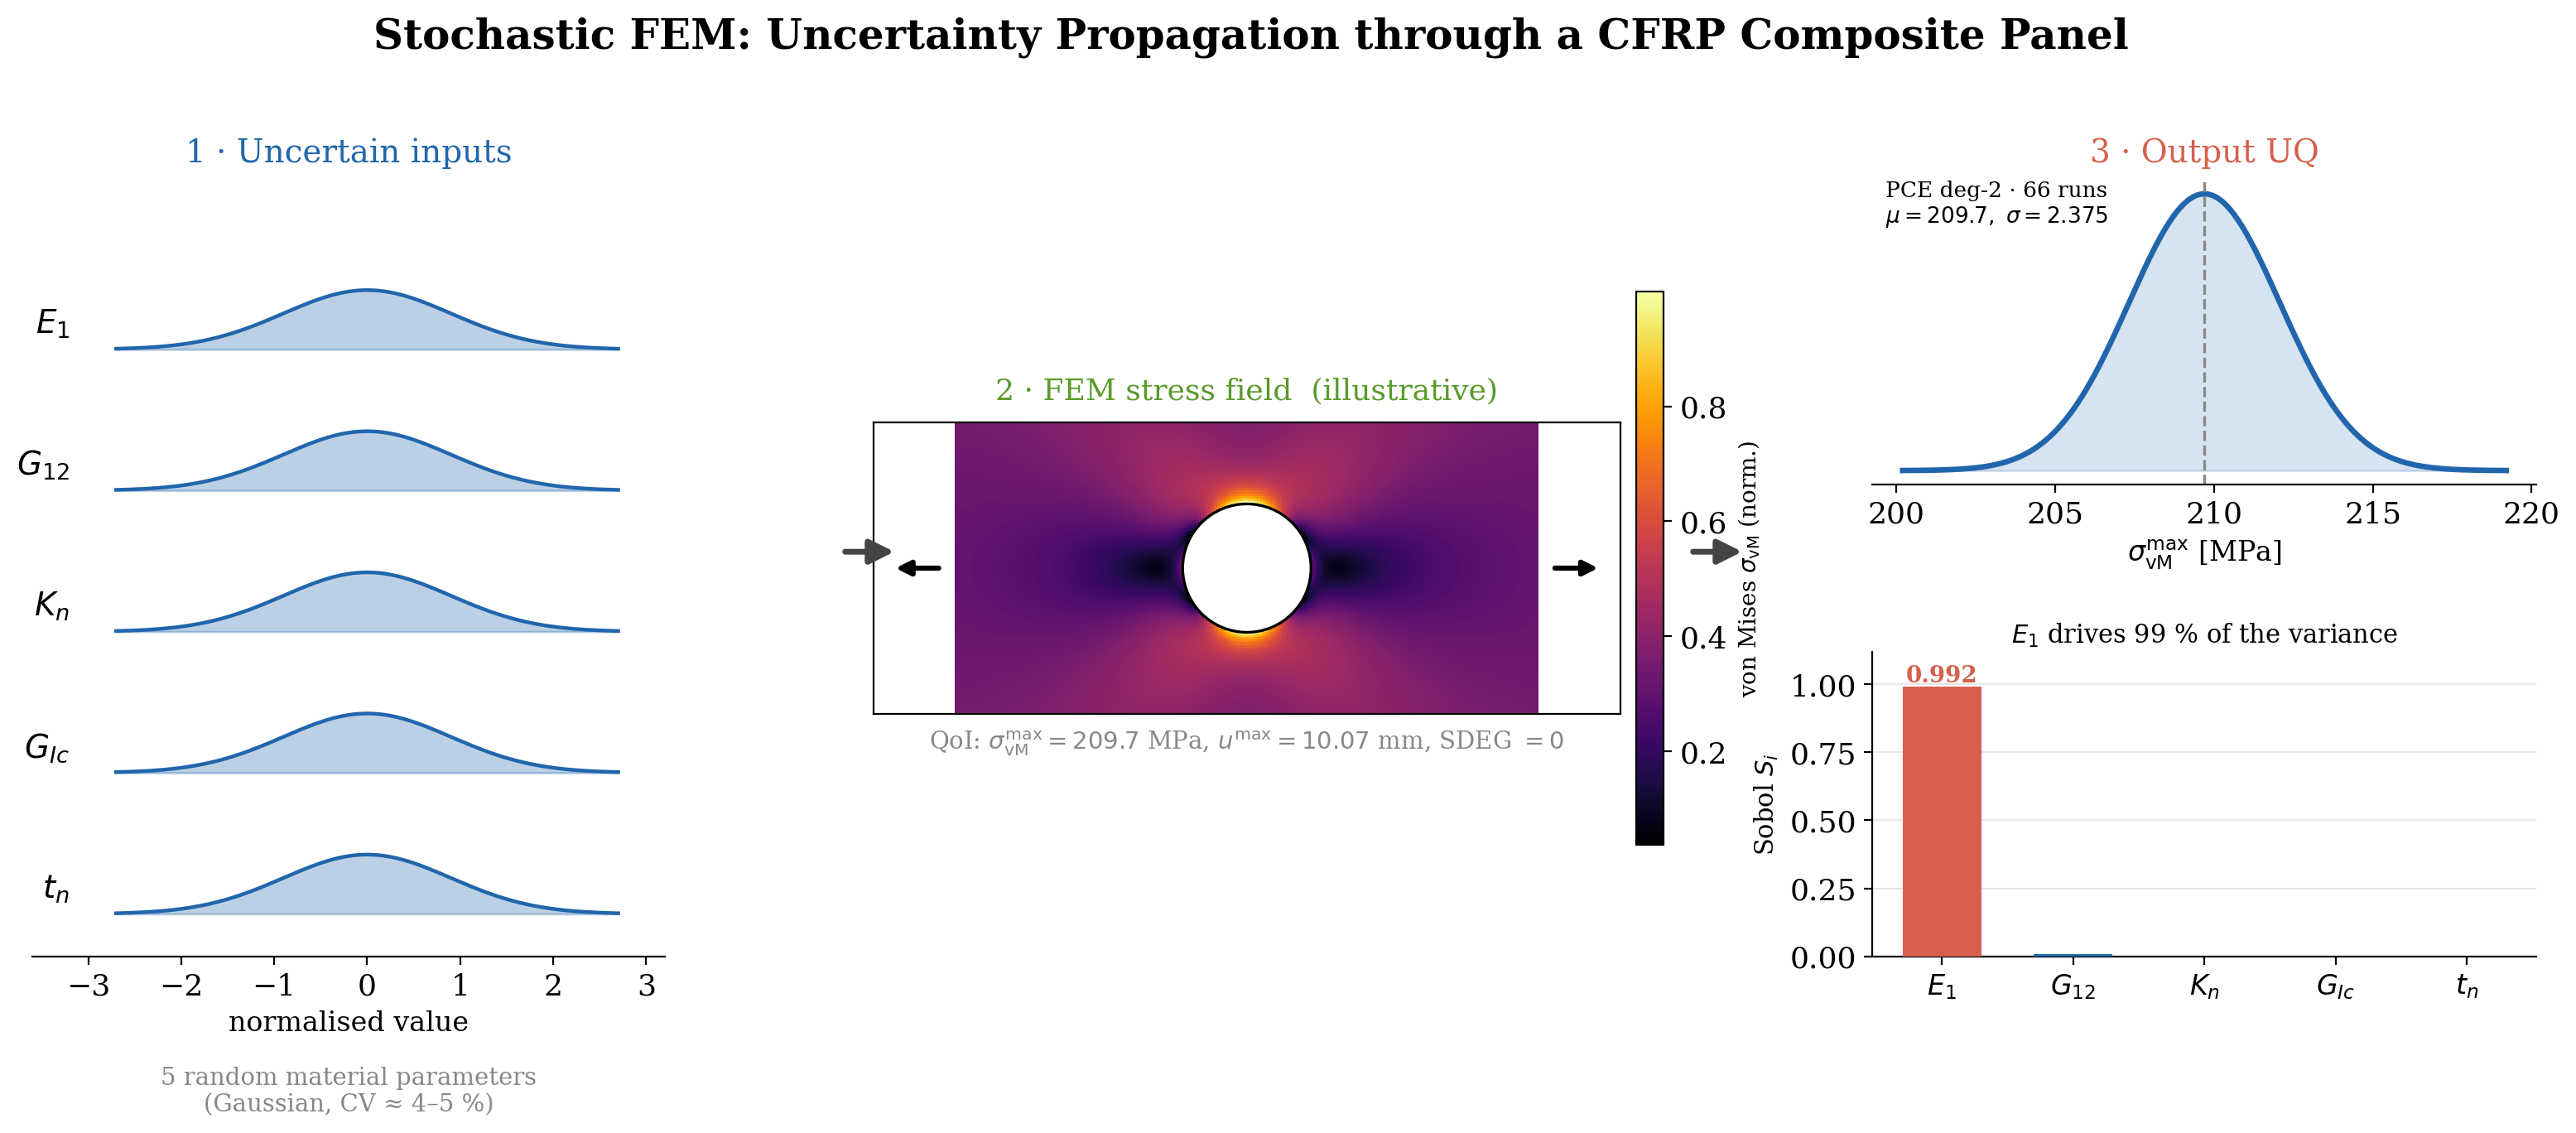
\includegraphics[width=0.96\linewidth]{hero_sfem_pipeline.png}
\end{center}

\section*{1. 概要}
JAXA H3ロケットのペイロードフェアリング（CFRP表皮＋アルミハニカムコアのサンドイッチ）を対象に、
\textbf{製造で生じる材料ばらつきが構造応答へどう伝播するか}を定量化した。
高忠実度のAbaqusモデルを\textbf{ブラックボックス}として扱い、
\textbf{非侵入型の多項式カオス展開（PCE）}を確率有限要素法のサロゲートとして構築した。

\section*{2. 背景と目的}
CFRPと接着層の物性は、繊維体積率・硬化条件・接着フィルム厚などの製造要因で本質的にばらつく。
このばらつきは応力・損傷・変形、ひいては信頼性に伝播する。目的は次の4点：
\begin{enumerate}\itemsep1pt
  \item Smolyakスパース求積による\textbf{2次・3次PCE}の構築と収束検証
  \item \textbf{Sobol感度解析}による支配パラメータの同定
  \item 破壊確率 $P_f$ と信頼性指標 $\beta$ による\textbf{信頼性評価}
  \item PCEと\textbf{ニューラルネット（NN）}サロゲートの精度・解釈性比較
\end{enumerate}

\section*{3. 手法}
応答 $Y=\mathcal{M}(\xi)$ を $Y\approx\sum_{\alpha}c_\alpha\Psi_\alpha(\xi)$ とエルミート多項式で展開。
直交性から\textbf{平均・分散・Sobol指数が係数から解析的に}得られ、追加解析が不要。
各求積点で.inpの材料カードを書き換えてAbaqusを実行し、QoIを\texttt{odbAccess}で抽出してPCE係数を回帰。

\section*{4. 解析モデル}
CFRP表皮（直交異方LAMINA）＋アルミハニカムコア＋接着界面（\textbf{凝集域モデル CZM}、BK混合モード）。
2ステップ静荷重。\textbf{5つの不確定入力}：表皮の $E_1, G_{12}$、接着の $K_n, G_{Ic}, t_n$（変動係数約4--5\%、切断正規分布）。
QoIは最大von Mises応力（限界1{,}200\,MPa）・最大CZM損傷SDEG（限界0.5）・最大変位。

\section*{5. 主な結果}
\begin{itemize}\itemsep1pt
  \item \textbf{2次PCE（66回）で統計量が収束}：3次（286回）と4桁一致。
  \item \textbf{$E_1$ が出力分散の99\%超を支配}（Sobol $S_{E_1}=0.992$）。他は実質寄与なし。
  \item \textbf{広い安全余裕}：$\sigma_\mathrm{vM}^{\max}=209.7\pm2.38$\,MPa $\ll$ 1{,}200\,MPa、
        $P_f\approx0$、$\beta$ は実質無限大。
  \item \textbf{SDEG $\equiv 0$}：全試行で接着損傷は発生せず（この荷重では接着パラメータは構造的に同定不能）。
  \item \textbf{PCEがNNより高精度}（この滑らかな応答ではPCEの低次多項式の事前知識が有効）。
\end{itemize}

\begin{table}[h]\centering\small
\begin{tabular}{lccc}
\toprule
QoI & 平均 & 標準偏差 & 変動係数 \\
\midrule
最大von Mises応力 & 209.7\,MPa & 2.375\,MPa & 1.13\,\% \\
最大変位          & 10.07\,mm  & 0.178\,mm  & 1.76\,\% \\
最大SDEG          & 0.000      & 0.000      & ---       \\
\bottomrule
\end{tabular}
\end{table}

\section*{6. 結論}
本研究は、製造ばらつき下のH3フェアリングについて、わずか66回の決定論的解析から
\textbf{応答統計・支配因子・信頼性}を一貫して導いた。実務的含意は明快で、
\textbf{$E_1$ の品質管理を締めることが最も効果的}である。一方、現荷重では接着パラメータが同定不能であり、
損傷を励起する高荷重・損傷進展シナリオが今後の課題である。

\vfill
{\footnotesize ※本要約は確率有限要素法レポート（\texttt{report\_paper.pdf}）の簡易版。図中の応力場は概念図で、
数値（平均209.7/標準偏差2.375/Sobol $E_1=0.992$）は実結果。}

\clearpage
\section*{7. 分かりやすいストーリー版（スライド順・口頭直前用）}

\paragraph{ひとことで言うと}
ロケットのフェアリング（CFRP外皮＋アルミハニカム）は製造で材料がバラつく。そのバラつきが応力に
どう響くかを、Abaqusを黒箱のままPCEで効率よく調べた。結論：\textbf{$E_1$（繊維方向の硬さ）だけで
99\%決まる。構造は広い余裕で安全。}

\begin{description}\itemsep2pt
  \item[① 動機] フェアリングはCFRP外皮＋ハニカムの板。製造（繊維量・硬化・接着厚）で材料がバラつき、
        応力・損傷・たわみ、ひいては信頼性に効く。\emph{そのバラつきを定量化したい}。
  \item[② 何を不確かとみなすか] 5つの材料パラメータ：外皮の $E_1$（繊維方向剛性）・$G_{12}$（面内せん断）、
        接着の $K_n,G_{Ic},t_n$。各々ガウスだが正値なので $\pm50\%$ で打ち切り。
  \item[③ 手法の核] \textbf{PCE}＝応答を直交多項式の和で近似（入力ガウス→Hermite基底）。
        ご利益は\textbf{平均$=c_0$、分散$=$係数の二乗和、Sobolも係数から即出る（追加計算ゼロ）}。
        \textbf{Smolyakスパース求積}で本来1024回のAbaqusを\textbf{66回(2次)/286回(3次)}に削減。
  \item[④ FEモデル] 外皮=直交異方弾性、コア=弾性、接着=\textbf{凝集域モデル(CZM, BK則)}。
        2段階荷重で解き、QoI（ミーゼス応力・損傷SDEG・変位）を最終フレームから抽出。
  \item[⑤ 結果1：収束] 2次(66回)と3次(286回)が\textbf{有効数字4桁で一致}→2次で十分。
        応力 $209.7\pm2.38$\,MPa（バラつき1.1\%）。\textbf{損傷SDEGは全352回ゼロ}。
  \item[⑥ 結果2：$E_1$支配（山場）] Sobol $S_{E_1}=0.992$。なぜ？→
        $\mathrm{Var}(Y)\approx\sum(\partial Y/\partial\xi_i)^2\sigma_i^2$。板は膜で荷重を受け、応力は$E_1$が
        直接決める（感度大）うえ$E_1$自身も5\%ばらつく。$G_{12}$はばらつき2倍でも感度小で潰れる。
        \emph{最もバラつく入力でなく、構造が増幅する入力が効く}。
  \item[⑦ 結果3：PCE vs NN] PCEが高精度。NNはサンプルを66→286に増やすと誤差が1桁悪化（過学習）。
        一般論でなく\emph{「滑らか＝低次多項式」という正しい事前知識をPCEが持つから勝った}。
  \item[⑧ 信頼性] 平均応力は破壊限界の\textbf{約416$\sigma$下}→$P_f\approx0,\ \beta\approx\infty$。ただし
        \textbf{「解析の分解能以下」}と言う（MCは$10^{-6}$まで、入力$\pm50\%$打ち切りで外挿不可）。
        SDEG$\equiv0$ゆえ接着パラメータは\textbf{構造的に同定不能}＝5次元が実質1次元($E_1$)に縮退。
  \item[⑨ 結論＆限界] \textbf{$E_1$の品質管理を締めるのが最も効果的}（唯一の実務メッセージ）。
        限界：$P_f=0$は分解能限界／入力独立仮定（実際は相関）／単一パネル／接着を損傷させる
        荷重ケースが今後の課題。
\end{description}

\section*{8. 口頭で刺さる「3つの一言」}
\begin{enumerate}\itemsep2pt
  \item \textbf{直交性のおかげで統計量とSobolが係数からタダで出る}（＝PCEを選んだ理由）。
  \item \textbf{ランキングは「最もバラつく入力」でなく「構造が増幅する入力」で決まる}（＝$E_1$支配の物理）。
  \item \textbf{$P_f=0$は保証でなく「分解能以下」。SDEG$=0$は知見であってバグではない}（＝誠実さの提示）。
\end{enumerate}

\end{document}
